% Provenance (never printed): cycle 2 "Questionner l'espace et le temps"
% (oceans, seas, continents on the globe) and "Questionner le monde de la
% matiere" (states of water in natural phenomena); see sources/book1/PROVENANCE.md.
% Book 1, grade 2, chapter 1.
\chapter{El agua en la Tierra}\label{ch:g2:water-on-earth}

El 7 de diciembre de 1972, tres astronautas que viajaban hacia la Luna
giraron su cámara hacia la Tierra. Su fotografía se convirtió en una de las
imágenes más famosas que se han tomado jamás. Mírala. Se ven nubes blancas,
un poco de tierra marrón y amarilla, el hielo blanco abajo --- y azul, azul
por todas partes. Vista desde el espacio, nuestra Tierra es un planeta azul.

\begin{omfigure}
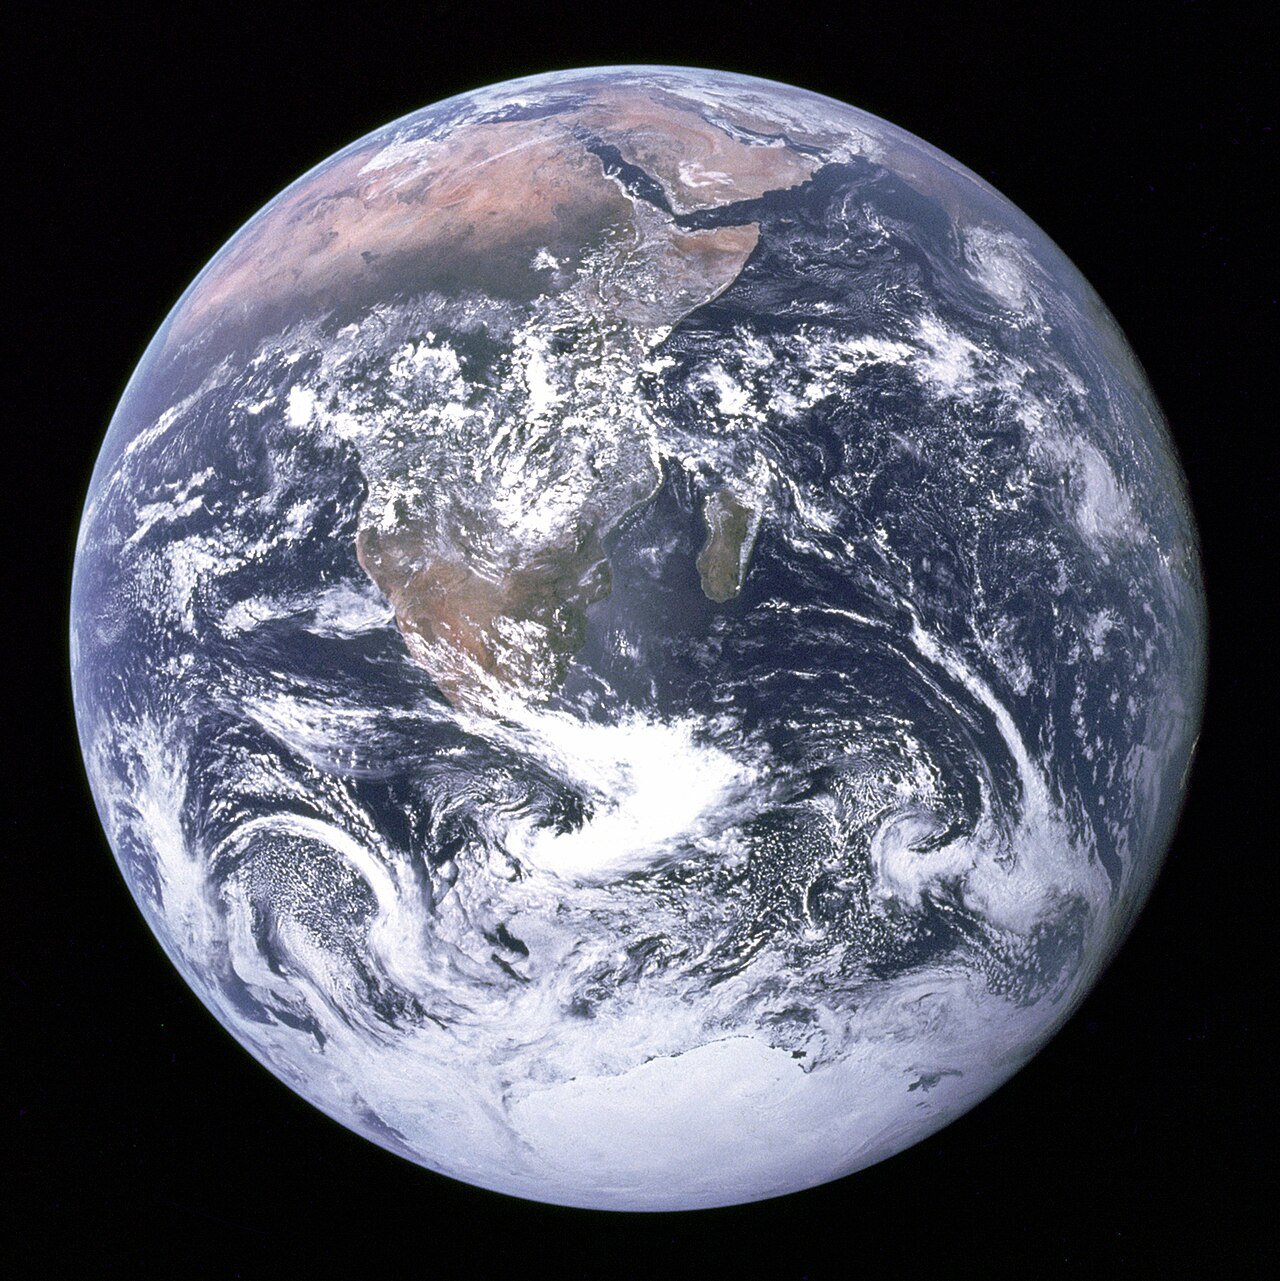
\includegraphics[width=0.5\linewidth]{images/book1/g2-nasa-blue-marble.jpg}

{\small La Tierra fotografiada por la tripulación del Apolo~17, el
7~de diciembre de 1972. Se ven África, Arabia arriba y el hielo de la
Antártida abajo. Fotografía: NASA (dominio público).}
\end{omfigure}

\begin{recall}
El agua puede ser un sólido (el hielo), un líquido o un gas que no vemos (el
vapor de agua). El agua líquida que se deja al sol se convierte poco a poco
en vapor: se evapora. Cuando el vapor se enfría, vuelve a convertirse en
gotitas: se condensa. Ya has visto estos cambios en los libros de física. En
un \omterm{def:g1:landscapes-around-us:landscape}{paisaje}, el agua corre por los \omterm{def:g1:landscapes-around-us:water}{ríos} y se queda en los \omterm{def:g1:landscapes-around-us:water}{lagos}
(\cref{ch:g1:landscapes-around-us}).
\end{recall}

\section{El planeta azul}

Casi toda la Tierra está cubierta de agua. Imagina toda la superficie de la
Tierra cortada en 100 cuadrados iguales. Si pintamos de azul cada cuadrado
cubierto por el \omterm{def:g2:water-on-earth:ocean}{mar}, pintamos 71 cuadrados. Solo 29 cuadrados son tierra.

\begin{omfigure}
\begin{tikzpicture}
  \begin{axis}[hide axis, width=7.2cm, height=7.2cm, xmin=-0.5, xmax=9.5,
      ymin=-0.5, ymax=9.5, axis equal image, scale only axis,
      clip=false]
    \addplot[scatter, only marks, mark=square*, mark size=9.2pt,
      scatter/classes={0={fill=green!45!omLithAlluv, draw=black!40},
                       1={fill=omSea!80!blue, draw=black!40}},
      point meta=explicit symbolic]
      table[x=col, y=row, meta=blue] {figdata/out/grade-2-ocean_fraction-grid.dat};
  \end{axis}
\end{tikzpicture}

{\small Si la superficie de la Tierra se cortara en 100 cuadrados iguales,
71 serían \omterm{def:g2:water-on-earth:ocean}{mar} (azul) y 29 serían tierra (verde). Calculado a partir de un
mapa del relieve de toda la Tierra (NOAA ETOPO1).}
\label{fig:g2:water-on-earth:grid}
\end{omfigure}
% ledger: data:etopo1, wss:ocean-cover (71 % computed in figdata/grade-2/ocean_fraction.py)

Las grandes extensiones de \omterm{def:g2:water-on-earth:salt-fresh}{agua salada} que cubren casi toda la Tierra
tienen nombre.

\begin{definition}[Océano y mar]\label{def:g2:water-on-earth:ocean}
Un \emph{océano}\index{oceano@océano} es una de las extensiones muy grandes
de \omterm{def:g2:water-on-earth:salt-fresh}{agua salada} que cubren casi toda la Tierra y se encuentran entre los
continentes. Un \emph{mar}\index{mar} es una extensión más pequeña de \omterm{def:g2:water-on-earth:salt-fresh}{agua
salada}, normalmente en el borde de un océano y en parte rodeada de tierra.
\end{definition}

Todos los \omterm{def:g2:water-on-earth:ocean}{océanos} están unidos entre sí: un barco podría navegar de
cualquier \omterm{def:g2:water-on-earth:ocean}{océano} a cualquier otro sin cruzar tierra. Sus nombres, y dónde
están en un globo terráqueo, se ven en el \cref{ch:g3:continents-and-oceans}.

\begin{omfigure}
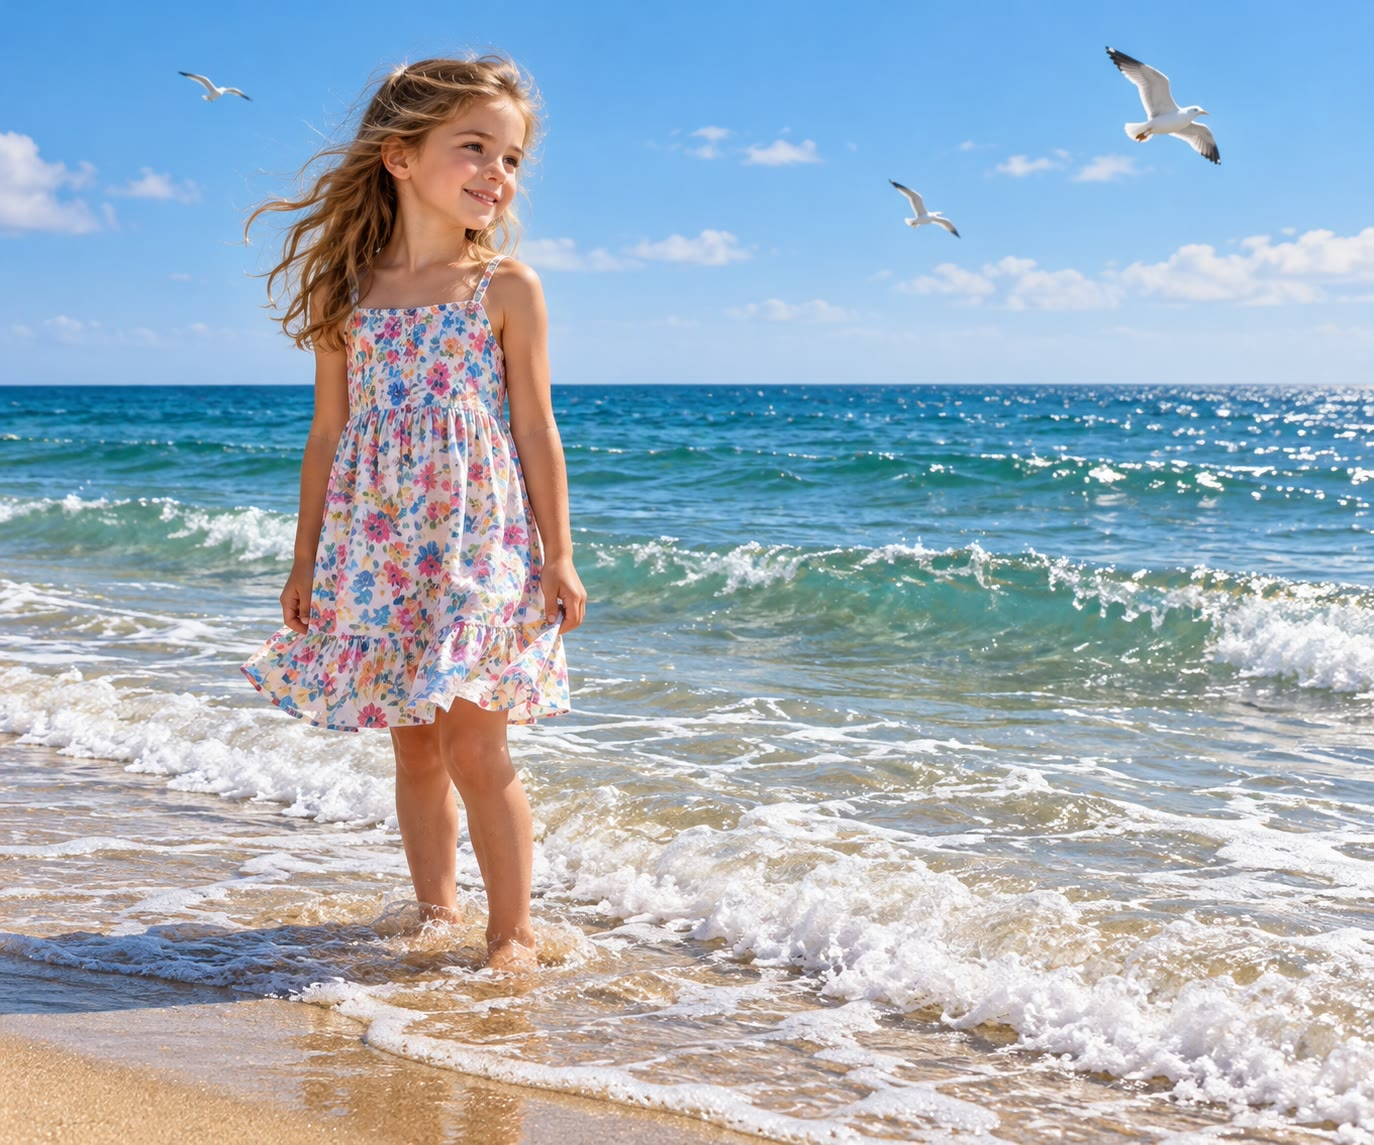
\includegraphics[width=0.62\linewidth]{images/book1/ai/g2-beach-sea.jpg}

{\small A la orilla del \omterm{def:g2:water-on-earth:ocean}{mar}. El agua sigue y sigue, mucho más lejos de lo
que alcanza la vista.}
\end{omfigure}

\section{Agua salada y agua dulce}

Si alguna vez has tragado un sorbo de agua de \omterm{def:g2:water-on-earth:ocean}{mar} mientras nadabas, ya lo
sabes: sabe muy salada. El agua de los \omterm{def:g1:landscapes-around-us:water}{ríos} y de los \omterm{def:g1:landscapes-around-us:water}{lagos}, no.

\begin{definition}[Agua salada y agua dulce]\label{def:g2:water-on-earth:salt-fresh}
El \emph{agua salada}\index{agua salada} tiene mucha sal disuelta: es el
agua de los \omterm{def:g2:water-on-earth:ocean}{océanos} y de los \omterm{def:g2:water-on-earth:ocean}{mares}. El \emph{agua dulce}\index{agua dulce}
tiene muy poca sal: es el agua de la lluvia, de casi todos los \omterm{def:g1:landscapes-around-us:water}{ríos} y \omterm{def:g1:landscapes-around-us:water}{lagos},
del hielo y de la nieve, y de los manantiales.
\end{definition}

\begin{example}[¿Cuánta sal tiene el mar?]\label{ex:g2:water-on-earth:salty}
% ledger: nos:salinity
En una botella con un kilogramo de agua de \omterm{def:g2:water-on-earth:ocean}{mar} --- más o menos un litro ---
hay unos 35 gramos de sal. Si dejamos que se evapore toda el agua, la sal se
queda en el fondo en forma de cristales blancos. Así se obtiene la sal
marina en las salinas junto al \omterm{def:g2:water-on-earth:ocean}{mar}, donde el sol y el viento secan poco a
poco unas balsas poco profundas de agua de \omterm{def:g2:water-on-earth:ocean}{mar}.
\end{example}

\begin{omfigure}
\begin{minipage}[b]{0.49\linewidth}\centering
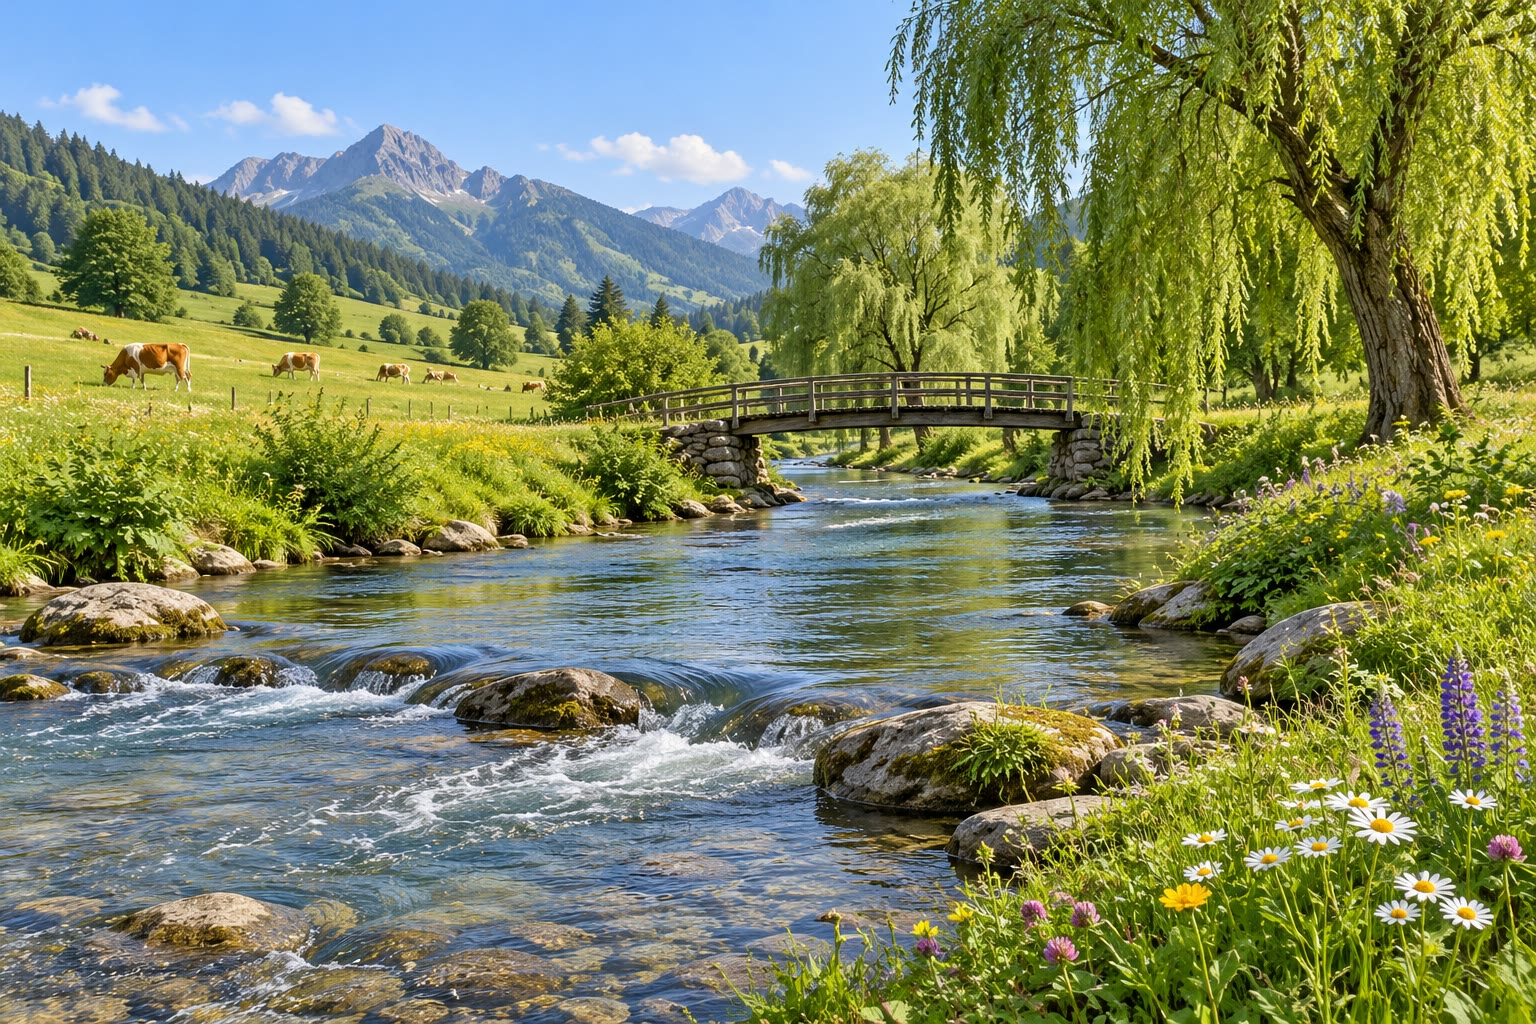
\includegraphics[width=\linewidth]{images/book1/ai/g2-river-meadow.jpg}

{\small \omterm{def:g2:water-on-earth:salt-fresh}{Agua dulce}: un \omterm{def:g1:landscapes-around-us:water}{río}.}
\end{minipage}\hfill
\begin{minipage}[b]{0.49\linewidth}\centering
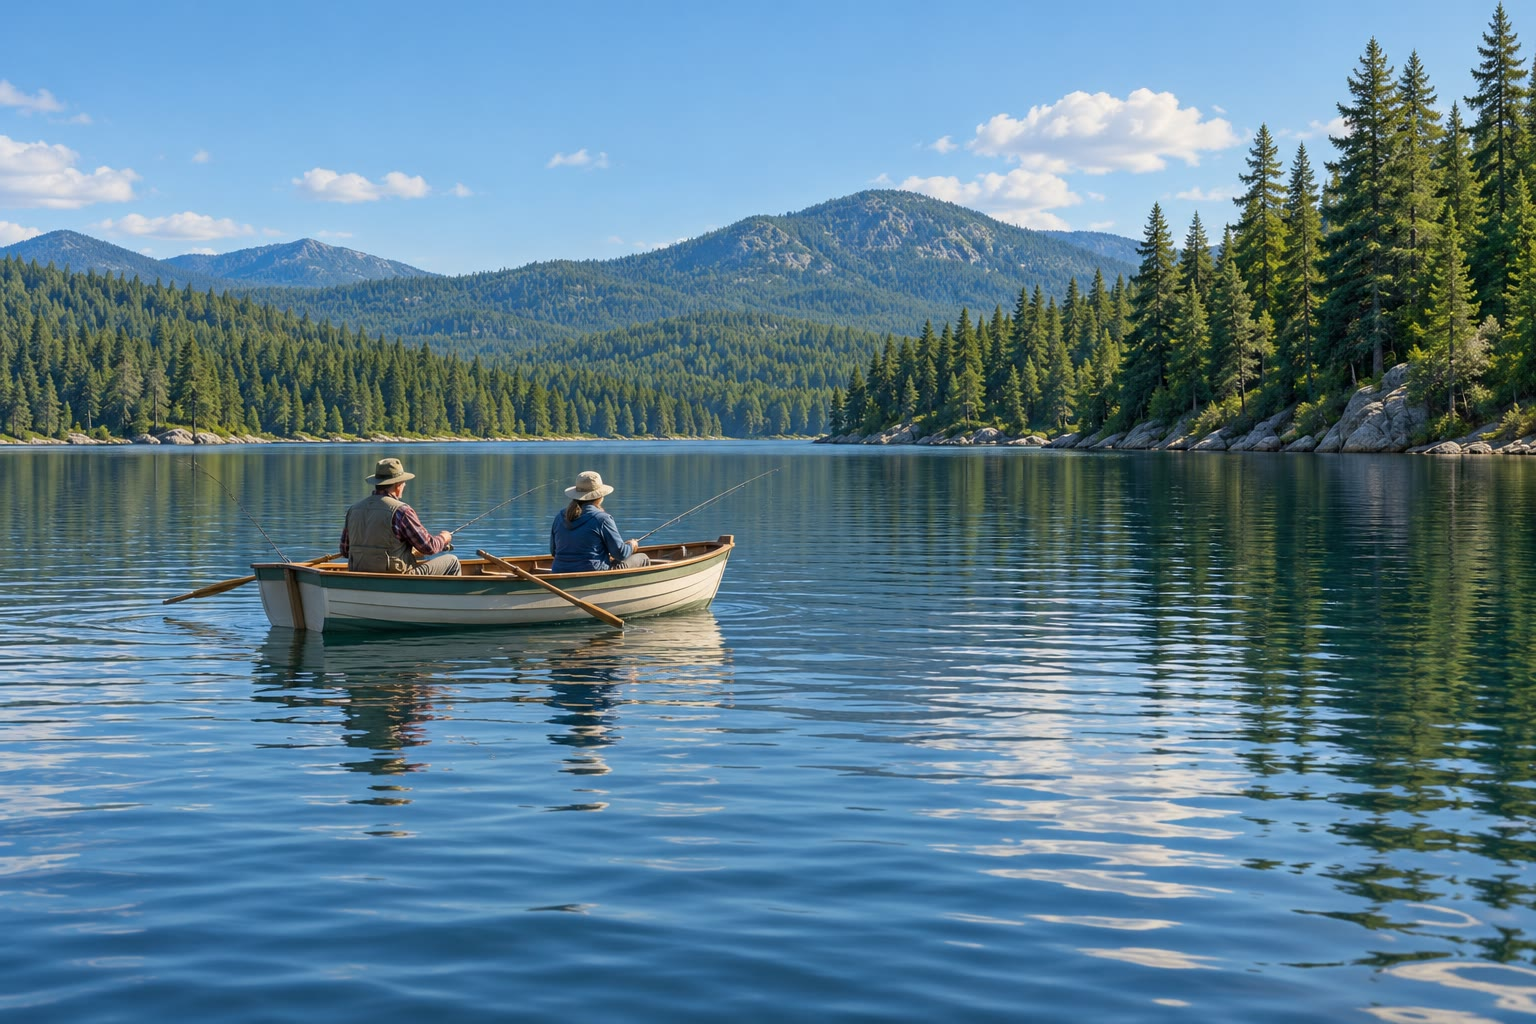
\includegraphics[width=\linewidth]{images/book1/ai/g2-lake-boat.jpg}

{\small \omterm{def:g2:water-on-earth:salt-fresh}{Agua dulce}: un \omterm{def:g1:landscapes-around-us:water}{lago}.}
\end{minipage}
\end{omfigure}

\begin{remark}[No podemos beber agua de mar]\label{rem:g2:water-on-earth:drink}
Las personas y los animales terrestres no pueden beber agua de \omterm{def:g2:water-on-earth:ocean}{mar}: tiene
demasiada sal, y beberla hace que el cuerpo pierda agua en lugar de
ganarla. Los marineros que navegan lejos, en alta \omterm{def:g2:water-on-earth:ocean}{mar}, rodeados de agua,
siempre han tenido que llevar consigo su \omterm{def:g2:water-on-earth:salt-fresh}{agua dulce}.
\end{remark}

\section{¿Dónde está toda el agua?}

El \omterm{def:g2:water-on-earth:salt-fresh}{agua dulce} no está solo en los \omterm{def:g1:landscapes-around-us:water}{ríos} y los \omterm{def:g1:landscapes-around-us:water}{lagos}. Una gran parte está
helada: en los grandes hielos blancos de la Antártida y de Groenlandia, y en
las altas \omterm{def:g1:landscapes-around-us:landform}{montañas}. Y otra gran parte está escondida bajo nuestros pies, en
el suelo, donde llena los diminutos huecos entre los granos de arena y las
grietas de la roca.

\begin{omfigure}
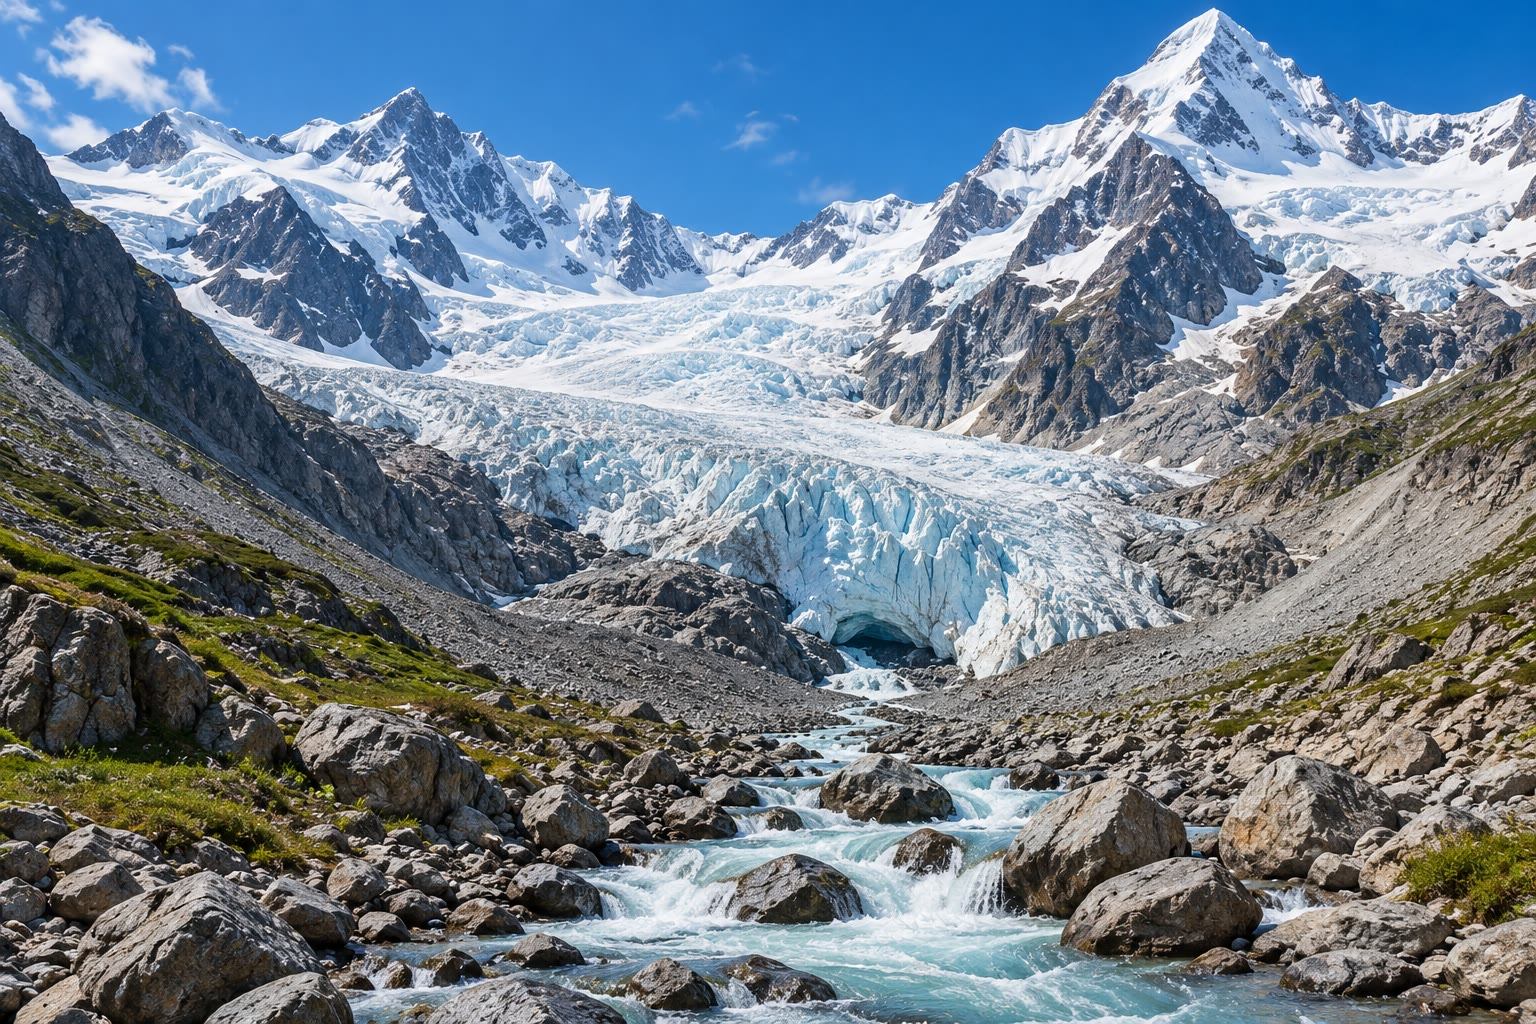
\includegraphics[width=0.62\linewidth]{images/book1/ai/g2-snowy-mountains.jpg}

{\small Las altas \omterm{def:g1:landscapes-around-us:landform}{montañas} guardan \omterm{def:g2:water-on-earth:salt-fresh}{agua dulce} en forma de nieve y de hielo
todo el año. En verano una parte se funde y alimenta los arroyos.}
\end{omfigure}

Imagina que pudiéramos echar toda el agua de la Tierra en 100 cubos del
mismo tamaño. ¿Cuántos cubos llenaría cada clase de agua?

\begin{omfigure}
\begin{tikzpicture}
  \begin{axis}[hide axis, width=7.2cm, height=7.2cm, xmin=-0.5, xmax=9.5,
      ymin=-0.5, ymax=9.5, axis equal image, scale only axis, clip=false]
    \addplot[scatter, only marks, mark=*, mark size=8pt,
      scatter/classes={0={fill=omSea!80!blue, draw=black!40},
                       1={fill=white, draw=black!60},
                       2={fill=brown!55, draw=black!40}},
      point meta=explicit symbolic]
      table[x=col, y=row, meta=kind] {figdata/out/grade-2-water_shares.dat};
  \end{axis}
  \begin{scope}[shift={(7.9,5.6)}, font=\small]
    \fill[omSea!80!blue, draw=black!40] (0,0) circle (0.2);
    \node[anchor=west] at (0.35,0) {agua salada de los océanos: 96 cubos};
    \fill[white, draw=black!60] (0,-0.7) circle (0.2);
    \node[anchor=west] at (0.35,-0.7) {hielo y nieve: 2 cubos};
    \fill[brown!55, draw=black!40] (0,-1.4) circle (0.2);
    \node[anchor=west] at (0.35,-1.4) {agua bajo el suelo: 2 cubos};
  \end{scope}
\end{tikzpicture}

{\small Toda el agua de la Tierra en 100 cubos. Los \omterm{def:g1:landscapes-around-us:water}{ríos}, los \omterm{def:g1:landscapes-around-us:water}{lagos}, las
nubes y el agua de todos los seres vivos juntos no llenarían ni un cubo.
Cifras del Servicio Geológico de Estados Unidos (USGS).}
\label{fig:g2:water-on-earth:buckets}
\end{omfigure}
% ledger: wss:water-shares (rounded to 100 buckets in figdata/grade-2/water_shares.py)

\begin{proposition}[Casi toda el agua de la Tierra es salada]\label{prop:g2:water-on-earth:most-salty}
% ledger: wss:water-shares
De 100 cubos con toda el agua de la Tierra, 96 son el \omterm{def:g2:water-on-earth:salt-fresh}{agua salada} de los
\omterm{def:g2:water-on-earth:ocean}{océanos}. El \omterm{def:g2:water-on-earth:salt-fresh}{agua dulce} que bebemos es solo una parte muy pequeña de toda el
agua: casi toda ella está helada en el hielo o escondida bajo el suelo.
\end{proposition}

\section{¿Adónde va la lluvia?}

Cuando llueve, el agua no se queda donde cae. Fíjate en el patio del colegio
después de un chubasco: una parte del agua corre por el suelo hasta las
alcantarillas, otra se mete en la tierra de los parterres, y los charcos
desaparecen poco a poco cuando vuelve a salir el sol.

\begin{omfigure}
\begin{tikzpicture}[x=1cm, y=1cm, font=\small]
  % sky, sea, land
  \fill[ocBlue!6] (0,0) rectangle (12,5.6);
  \fill[omSea] (8.6,0) rectangle (12,0.9);
  \fill[green!30!omLithAlluv] (0,0) -- (0,2.4) .. controls (2,2.6) and (3,2.0) .. (4.5,1.6)
     .. controls (6,1.2) and (7.5,1.0) .. (8.6,0.9) -- (8.6,0) -- cycle;
  % ground below the surface
  \fill[brown!25] (0,0) rectangle (8.6,0.6);
  % river
  \draw[omSea!70!blue, line width=2.4pt] (1.6,2.45) .. controls (3.5,2.0) and (6,1.15) .. (8.6,0.95);
  % cloud and rain
  \pic at (2.2,4.0) {puffycloud};
  \foreach \x in {1.4,1.8,2.2,2.6,3.0}
    \draw[omWxRain, line width=0.8pt] (\x,3.7) -- (\x-0.15,3.1);
  \pic at (9.6,4.3) {puffycloud};
  % arrows
  \draw[omWxRain, line width=1.1pt, -{Stealth[length=2.5mm]}] (3.3,2.15) -- (3.3,0.6);
  \node[anchor=west, align=left, font=\scriptsize] at (3.4,1.0) {una parte\\entra en el suelo};
  \draw[omWxRain, line width=1.1pt, -{Stealth[length=2.5mm]}] (5.4,1.55) -- (7.6,1.15);
  \node[align=center, font=\scriptsize] at (6.2,2.05) {otra corre hasta un río,\\y el río va al mar};
  \draw[black!50, line width=1.1pt, densely dashed, -{Stealth[length=2.5mm]}] (10.2,1.1) .. controls (10.4,2.4) and (10.1,3.2) .. (9.8,3.85);
  \node[align=left, anchor=west, font=\scriptsize] at (10.45,2.4) {el agua\\se evapora};
  \draw[black!50, line width=1.1pt, densely dashed, -{Stealth[length=2.5mm]}] (8.45,4.35) -- (3.6,4.3);
  \node[font=\scriptsize, above] at (6.0,4.35) {el viento lleva las nubes};
  \node[font=\scriptsize] at (10.4,0.45) {mar};
  \node[font=\scriptsize, anchor=west] at (0.2,3.25) {lluvia};
\end{tikzpicture}

{\small Adónde va la lluvia. El agua que sube del \omterm{def:g2:water-on-earth:ocean}{mar} y de la tierra en
forma de vapor forma nuevas nubes, y las nubes traen nueva lluvia.}
\label{fig:g2:water-on-earth:rain}
\end{omfigure}

\begin{method}[Seguir una gota de lluvia]\label{met:g2:water-on-earth:drop}
Para seguir una gota de lluvia, hazte tres preguntas, una tras otra:
\begin{enumerate}
  \item ¿Dónde cae: en el \omterm{def:g2:water-on-earth:ocean}{mar}, en un tejado, en el suelo, en una \omterm{def:g1:landscapes-around-us:landform}{montaña}?
  \item ¿Se mete en el suelo, corre por la superficie o se congela y se
        convierte en hielo?
  \item ¿Adónde va después: a un \omterm{def:g1:landscapes-around-us:water}{río}, a un \omterm{def:g1:landscapes-around-us:water}{lago}, al \omterm{def:g2:water-on-earth:ocean}{mar}, al suelo o de
        vuelta al aire?
\end{enumerate}
Al final, cada gota vuelve al \omterm{def:g2:water-on-earth:ocean}{mar} o al aire, y el viaje empieza otra vez.
\end{method}

\begin{example}[Una gota en la montaña]\label{ex:g2:water-on-earth:mountain}
Una gota de lluvia cae en forma de nieve en una alta \omterm{def:g1:landscapes-around-us:landform}{montaña} en invierno.
Se queda allí, helada, hasta los días cálidos del verano. Entonces se
funde, baja hasta un arroyo de \omterm{def:g1:landscapes-around-us:landform}{montaña}, llega a un \omterm{def:g1:landscapes-around-us:water}{río}, y el \omterm{def:g1:landscapes-around-us:water}{río} la lleva
al \omterm{def:g2:water-on-earth:ocean}{mar}. Un día de sol la gota se evapora del \omterm{def:g2:water-on-earth:ocean}{mar} y sube al aire, donde pasa
a formar parte de una nube nueva.
\end{example}

\section{Ejercicios}

\begin{exercise}[$\star$]\label{exo:g2:water-on-earth:1}
¿\omterm{def:g2:water-on-earth:salt-fresh}{Agua salada} o \omterm{def:g2:water-on-earth:salt-fresh}{agua dulce}? El \omterm{def:g2:water-on-earth:ocean}{mar}; un \omterm{def:g1:landscapes-around-us:water}{río}; la lluvia; un \omterm{def:g1:landscapes-around-us:water}{lago} de \omterm{def:g1:landscapes-around-us:landform}{montaña};
un \omterm{def:g2:water-on-earth:ocean}{océano}; el hielo de una \omterm{def:g1:landscapes-around-us:landform}{montaña}.
\end{exercise}

\begin{exercise}[$\star$]\label{exo:g2:water-on-earth:2}
¿Por qué llamamos a la Tierra el ``planeta azul''?
\end{exercise}

\begin{exercise}[$\star$]\label{exo:g2:water-on-earth:3}
En la cuadrícula de 100 cuadrados, 71 cuadrados son azules. ¿Cuántos
cuadrados son tierra?
\end{exercise}

\begin{exercise}[$\star$]\label{exo:g2:water-on-earth:4}
¿Qué es más grande, un \omterm{def:g2:water-on-earth:ocean}{océano} o un \omterm{def:g2:water-on-earth:ocean}{mar}?
\end{exercise}

\begin{exercise}[$\star$]\label{exo:g2:water-on-earth:5}
¿Puede un marinero en medio del \omterm{def:g2:water-on-earth:ocean}{océano} beber el agua que rodea su barco?
¿Por qué?
\end{exercise}

\begin{exercise}[$\star$]\label{exo:g2:water-on-earth:6}
Nombra tres lugares donde hay \omterm{def:g2:water-on-earth:salt-fresh}{agua dulce}.
\end{exercise}

\begin{exercise}[$\star\star$]\label{exo:g2:water-on-earth:7}
En el dibujo de los 100 cubos, ¿cuántos cubos son de \omterm{def:g2:water-on-earth:salt-fresh}{agua salada}? ¿Cuántos
son de \omterm{def:g2:water-on-earth:salt-fresh}{agua dulce} (el hielo y el agua bajo el suelo juntos)?
\end{exercise}

\begin{exercise}[$\star\star$]\label{exo:g2:water-on-earth:8}
Ordena de la que guarda más agua a la que guarda menos: los \omterm{def:g1:landscapes-around-us:water}{ríos}; los
\omterm{def:g2:water-on-earth:ocean}{océanos}; el hielo y la nieve.
\end{exercise}

\begin{exercise}[$\star\star$]\label{exo:g2:water-on-earth:9}
Llueve sobre un campo. Di dos cosas que le pueden pasar al agua.
\end{exercise}

\begin{exercise}[$\star\star$]\label{exo:g2:water-on-earth:10}
Se deja al sol durante muchos días un recipiente con agua de \omterm{def:g2:water-on-earth:ocean}{mar}, hasta que
el agua desaparece. ¿Qué queda en el fondo del recipiente? ¿Adónde ha ido el
agua?
\end{exercise}

\begin{exercise}[$\star\star$]\label{exo:g2:water-on-earth:11}
Cuenta el viaje de una gota de lluvia que cae en el tejado del colegio,
hasta que vuelve a estar en una nube.
\end{exercise}
